\documentclass[11pt,a4paper]{article}

\usepackage{geometry} \geometry{left=2.2cm, right=2.2cm, top=2.2cm, bottom=2cm}
\parskip 0.15cm 
\setlength{\parindent}{0cm} 
\usepackage{pdflscape}
\usepackage[document]{ragged2e}

\usepackage[T1]{fontenc}  % Set font

\usepackage{lineno}  % Line numbers

\usepackage{amssymb}  % Symbols
\usepackage{amsmath}
\usepackage{siunitx}
\usepackage{textcomp}
\newcommand{\textapprox}{\raisebox{0.5ex}{\texttildelow}}  % Command for a good tilde

\linespread{1.5}  % Linespacing

\usepackage{xcolor} \newcommand{\TODO}[1]{\textcolor{red}{\textbf{#1}}}   %

\usepackage{lineno}

% Tables
\usepackage{multirow} \setlength{\tabcolsep}{4pt}

% Image handling
\usepackage{graphicx} 

\makeatletter \g@addto@macro\@floatboxreset\centering  
\makeatother

\graphicspath{ {img/} }  % Define image path

\usepackage{subfig}  % Compound figures

\usepackage{float}  % Precise figure location

% Bibliography management
\usepackage[style=authoryear, natbib=true, backend=biber]{biblatex}
\addbibresource{workflow.bib}

% Links within document, nice figure formatting
\usepackage[breaklinks]{hyperref} \definecolor{links}{RGB}{0,0,0} \hypersetup{
	breaklinks, colorlinks=true, linkcolor=links, anchorcolor=links,
	citecolor=links, filecolor=links, menucolor=links, runcolor=links,
	urlcolor=links, pdfauthor={John L. Godlee} }
	\def\subsectionautorefname{section} \def\subsubsectionautorefname{section}

% Variables
\newcommand{\mispreps}{20}
\newcommand{\minreps}{100}
\newcommand{\minsp}{9}
\newcommand{\wireps}{20}
\newcommand{\wistart}{100}


\title{Estimation of woodland canopy structure with terrestrial LiDAR: expanded methods}
\author{John L. Godlee}
\date{}

% Body
\begin{document}

\maketitle{}

\tableofcontents{}

\linenumbers

\section{Introduction}

This document provides detailed field and analytical methods for the study of tree canopy structure in southern African woodlands. The study aimed to understand the effects of tree species diversity and stand structure on tree canopy structure and grass biomass. Chapter XXX contains the same methods in brief.

\section{Sampling}

Fieldwork was conducted at two sites, the first in Bicuar National Park, southwest Angola (S15.1$^\circ$, E14.8$^\circ$), and the second in and around Mtarure Forest Reserve, southeast Tanzania (S9.0$^\circ$, E39.0$^\circ$). Fieldwork was conducted during the peak growth period of each site, in order to capture the highest foliage volume in the canopy and grass volume in the understorey.

\begin{figure}[H]
\centering
	\includegraphics[width=\textwidth]{map}
	\caption{Location of study sites within southern Africa (a), and of 1 ha plots within each site. The black polygons denote the boundaries of protected areas which encompass the majority of study sites, Bicuar National Park in Angola (b), and Mtarure Forest Reserve in Tanzania (c). Each site map is coloured according to the GlobCover global land cover classification.}
	\label{map}
\end{figure}

% latex table generated in R 4.0.2 by xtable 1.8-4 package
% Mon Apr 19 15:00:00 2021
\begin{table}[H]
\centering
\begin{tabular}{rcccc}
  \hline
{Site} & \multicolumn{1}{p{2.5cm}}{\centering MAT \\ (\textdegree{}C)} & \multicolumn{1}{p{2.5cm}}{\centering MAP \\ (mm y\textsuperscript{-1})} & \multicolumn{1}{p{2.5cm}}{\centering Temp. range \\ (\textdegree{}C)} & \multicolumn{1}{p{2.5cm}}{\centering CWD \\ (mm y\textsuperscript{-1})} \\
  \hline
Bicuar & 20.8 (0.70) & 825.9 (52.01) & 24.5 (0.90) & -844.8 (44.29) \\ 
  Mtarure & 25.7 (0.24) & 958.4 (25.19) & 12.0 (0.33) & -739.6 (8.06) \\ 
   \hline
\end{tabular}
\caption{Climatic data for each site, extracted from WorldClim at 2.5 minute resolution. Values are the mean and standard deviation (in brackets) of all pixels intersecting each protected area. MAT = Mean Annual Temperature. MAP = Mean Annual Precipitation. Temp. range = Temperature range, calculated as the mean of annual difference between highest temperature of hottest month and lowest temperature of coldest month. CWD = Climatic Water Deficit, calculated as the sum of the difference between monthly rainfall and monthly evapotranspiration when the difference is negative, sensu \citet{Chave2014}.} 
\label{clim}
\end{table}



At each site, a number of 1 ha permanent plots were sampled. In Angola, 15 plots were sampled, while in Tanzania, only seven were sampled, following the curtailment of fieldwork due to COVID-19 travel restrictions. Permanent plots were located in areas of homogeneous vegetation type, away from roads and undisturbed by humans. Plots were established following the SEOSAW protocol (version 3.0, \citealt{SEOSAW2020}). Plots were located quasi-randomly by first locating areas from satellite imagery expected to comprise savanna woodland vegetation. At each site, plots were deliberately located along a gradient of stem density.

Each permanent plot was further subdivided into nine 10 m diameter circular subplots arranged in a regular grid, with a buffer from the plot edge (\autoref{subplot}).

\begin{figure}[H]
\centering
	\includegraphics[width=\textwidth]{subplot}
	\caption{The layout of 10 m diameter subplots within each 1 ha square plot. Each subplot is situated inside a 15 m buffer from the plot edge, with 35 m between subplot centres. Subplots are arranged in a 3x3 grid. Disc-pasture measurements and biomass samples are located in cardinal directions 2 m from the centre of the subplot. All distances are in metres.}
	\label{subplot}
\end{figure}

\section{Field measurements}

\subsection{Trees}

For each subplot, we measured all woody stems >5 cm stem diameter with canopy material inside the subplot. For each stem we recorded:

\begin{itemize}
	\item{Tree identity}
	\item{Stem diameter (diameter at breast height - 1.3 m)}
\end{itemize}

For each tree, which may be composed of multiple stems joined at the base, we recorded: 

\begin{itemize}
	\item{Species}
	\item{Height to top of canopy}
	\item{Canopy area, ellipse from two perpendicular measurements (\autoref{crown})}
	\item{Distance from subplot centre}
	\item{Compass direction from subplot centre}
\end{itemize}

\begin{figure}[H]
\centering
	\includegraphics[width=\textwidth]{crown}
	\caption{Examples of tree crowns as viewed from above to demonstrate how crown extent measurements are located. Darker grey circles show the main stem while pale grey polygons show the maximum extent of the crown. Extent measurements are taken parallel to the plot edges. a) shows a perfectly circular tree crown, b) and c) show irregular tree crowns, demonstrating that maximum crown extent in a given orientation be offset from the stem.}
	\label{crown}
\end{figure}

\subsection{Grass biomass} 

Grass volume and biomass within each subplot was estimated from four sample points located 2 m from the subplot centre in cardinal directions (\autoref{subplot}). At each point, a disc-pasture meter measurement was taken with a 45.8 cm radius disc weighing exactly 1.5 kg \citep{Bransby1977}. Small woody stems were removed from disc-pasture sample points before the disc-pasture measurement was taken. The location of the sample point was moved if the designated point intersected with coarse woody debris, rocks, shrubs, or standing trees. Within each 1 ha plot, biomass harvesting was conducted at nine randomly allocated disc-pasture sample points. Tree leaf litter was removed from biomass samples. Biomass harvesting involved clipping all grass material within the 45.8 cm radius to ground level, taking care not to include roots. Grass samples from Angola were dried until the mass remained constant ($\pm$5 g) for >48 hours, then weighed to ascertain the grass biomass. Grass samples from Tanzania could not be processed due to curtailment of fieldwork due to COVID-19 travel restrictions. 

\subsection{Hemispherical photography}

At the centre of each subplot a single photograph was taken with a Nikon D750 full-frame DSLR camera, with a circular fisheye lens. The lens had an equisolid (equal area) projection, which avoids image distortion. The projection function is given by: 

\begin{equation}
	R = 2f \sin{(\theta{}/2)}
\end{equation}

Where $R$ is the radial position of a point on the image on the sensor, $f$ is the focal length of the lens, and $\theta{}$ is the angle in radians of the desired angular radius of the cropped image. 

The photo was taken facing directly to zenith, with the top of the camera facing magnetic north, at a height of 1.3 m or above understorey vegetation, whichever was higher. \autoref{camera_settings} shows describes the camera settings for each hemispherical photo.

\begin{table}[H] \centering 
  \caption{Description of camera settings used for each hemispherical photo. Note that the values of shutter speed and ISO are deliberately variable within sensible thresholds to adapt to light conditions.} 
  \label{camera_settings} 
\begin{tabular}{@{\extracolsep{0pt}} rl} 
\\[-1.8ex]\hline 
\hline \\[-1.8ex] 
{Setting} & {Value} \\
\hline \\[-1.8ex] 
Camera model & Nikon D750 \\
Lens model & Sigma 8 mm f/3.5 EX DG Circular Fisheye \\
Pixel pitch & \SI{5.95}{\micro\meter} \\
Sensor resolution & 24.3 MP \\
Shutter speed & >1/60s \\
Aperture & 5-7 \\
ISO & 100-200 \\
Exposure compensation & -0.7 \citep{Brusa2014} \\
Focus & $\infty$ \citep{Hu2009, Frazer2001}\\
Image size & Large Fine JPEG - circular image 4016x4016 px \\
Orientation & Landscape \\
\hline
\hline \\[-1.8ex] 
\end{tabular} 
\end{table} 

Photos were captured under uniform light conditions as much as possible, either under overcast skies or early in the day before direct sunlight could be seen on the photo. 

ImageJ (Fiji version 2.1.0/1.53c) was used to binarize hemispherical photos \citep{}, to separate plant material from sky. We first split each image into red, green and blue channels. We used the Huang algorithm \cite{} to automatically threshold images, using the blue channel only, under the assumption that plant material reflects little blue light, while the sky reflects much more \citep{}. Images were saved as PNG at the original pixel resolution.

\subsection{Stand structure}

From the stem measurements we calculated a number of indices to characterise whole-plot and subplot stand structure.

We calculated the mean of the spatial mingling index ($M_{i}$) according to \citet{Gadow2002} at the plot level, with the adjustment for potential neighbourhood species pool suggested by \citet{Hui2011}. The spatial mingling index is a spatially explicit estimate of the degree to which species are spatially mixed within a plot:

\begin{gather}
	M = \overline{M_{i}} \\
	M_{i} = \frac{S_{i}}{n_{\text{max}}} \frac{1}{k} \sum_{j=1}^{k} v_{j} \\
	\text{with}\ v_{j} = \begin{cases}
		0,& \text{neighbour $j$ same species as reference $i$} \\
		1,& \text{otherwise}
	\end{cases} \\
\end{gather}

where $k$ is the number of nearest neighbours considered for each reference tree, $S_{i}$ is the number of species found among the $k$ nearest neighbours of tree $i$, $n_{\text{max}}$ is the potential number of species in the neighbourhood, i.e. $k + 1$, and $N$ is the total number of trees in the plot. In our case we used the conventional value of $k = 4$ \citep{Gadow2002, Hui2004, Hui2007}. The value of $M_{i}$ increases with greater mixing of species, and all else being equal will increase with number of species within the plot (\autoref{mingling_both}).

\begin{figure}[H]
\centering
	\includegraphics[width=\textwidth]{mingling_both}
	\caption{The behaviour of $M_{i}$ with increasing number of species (left), and increasing spatial mixing of species. The left panel was generated by randomly assigning different numbers of species, in equal proportions, to an evenly spaced grid of individuals. \mispreps{} replicates were conducted for each number of species. The right panel was generated by randomly swapping pairs of individuals in a plot with \minsp{} species arranged in mono-specific square blocks in an evenly spaced grid. Each line shows a single replicate, where individuals were swapped in an additive fashion, with \minreps{} total.} 
	\label{mingling_both}
\end{figure}

We also calculated the mean of the winkelmass $W_{i}$ according to \citet{Gadow2002} at the plot level. The winkelmass estimates the degree of spatial uniformity in stem spatial distribution:

\begin{gather}
	W = \overline{W_{i}} \\
	W_{i} = \frac{1}{k} \sum_{j=1}^{k} v_{j} \\
	\text{with}\ v_{j} = \begin{cases}
		0,& \alpha_{j} \le \alpha_{0} \\
		1,& \text{otherwise}
	\end{cases} \\
\end{gather}

where $\alpha_{j}$ is the angle between consecutive neighbours and $\alpha_{0}$ is the critical angle, where $\alpha_{0} = 360 / k$. The value of the winkelmass increases with increasing spatial clumping (decreasing spatial regularity) of individuals (\autoref{wi_diagram}), and in a plot with random tree distribution will increase as more neighbours are considered (\autoref{wi_k}).

\begin{figure}[H]
\centering
	\includegraphics[width=\textwidth]{winkelmass}
	\caption{Possible values of $W_{i}$ at a sample point $i$, denoted by a cross. Neighbours are represented as circles numbered sequentially from 1 to 4, where $k = 4$. The angles of arrows in each example are given below, along with the winkelmass for that example.}
	\label{winkelmass}
\end{figure}

\begin{figure}[H]
\centering
	\includegraphics[width=\textwidth]{wi_diagram}
	\caption{Variation in winkelmass with increasing spatial irregularity of individuals. The top panel shows variation of winkelmass in \wireps{} plots as individuals are sequentially moved to a random location within the plot. Red dotted lines correspond to the panels below which show the spatial distribution of individuals after a given number of random individual movements.}
	\label{wi_diagram}
\end{figure}

\begin{figure}[H]
\centering
	\includegraphics[width=\textwidth]{wi_k}
	\caption{Variation in winkelmass with increasing number of neighbours $k$ considered in the calculation. \wikn{} replicate plots were used, each with \wiki{} individuals randomly distributed in space.}
	\label{wi_k}
\end{figure}

To estimate tree spatial structure in subplots we used an adapted version of the Iterative Hegyi index ($H_{i}$) \citep{Hegyi1974}. Our adapted formula allows the index to be based on a point rather than a focal tree, transforming it from a tree-centric competition index to a point-centric crowding index:

\begin{equation}
	H_{i} = log\sum_{j=1}^{n} (\frac{1}{L_{ij}} D_{j})
\end{equation}

where $D_{j}$ is the stem diameter of neighbour tree $j$ and $L_{j}$ is the distance of the neighbour from the subplot centre.


\section{Terrestrial LIDAR}

Within each subplot, a variable number of scans were recorded using a Leica HDS6100 phase-shift terrestrial laser scanner (TLS). The number and position of scans within a subplot was determined by the arrangement and density of canopy material in the subplot. Scan positions were arranged to minimise shadows within the canopy, and to maximise canopy penetration. Number of scans per subplot ranged between one and five in both Angola and Tanzania (\autoref{scan_settings}).

Five Leica 6" planar tilt and turn cross-pattern reflective targets were used at each subplot to align scans. To allow registration of scans among subplots, the location of each target was registered using a Leica VIVA GS10 GNSS unit, set up in post-processed kinematic (PPK) configuration with a base-station located \textapprox{}100 m from the edge of each 1 ha plot. The location of each target was measured for at least 4 minutes. Further, we used the TrimbleRTX GNSS post-processing service to precisely locate each target \citep{Chen2011}. When registering scans we discarded targets with location accuracy of >3 cm. Scan registration for each subplot was conducted in Leica Cyclone (version 9.1). After registration, scan scenes were exported from Cyclone as PTX files, one per subplot.

\begin{table}[H] \centering 
  \caption{Description of scan settings used for each scan.} 
  \label{scan_settings} 
\begin{tabular}{@{\extracolsep{0pt}} rl} 
\\[-1.8ex]\hline 
\hline \\[-1.8ex] 
{Setting} & {Value} \\
\hline \\[-1.8ex] 
Scanner model & Leica HDS6100 \\
Wavelength & 650-690 nm \\
Spot size at exit & 3 mm \\
Beam divergence & 0.22 mrad \\
Range & 79 m @90\%; 50 m @18\% albedo \\
Azimuth range & 0-360\textdegree{} \\
Zenith range & 0-155\textdegree{} \\
Increments & 0.018\textdegree{} \\
Point spacing over 25 m & 7.9 mm \\
Pixels per line & 20000 \\
Lines & 10000 \\
Compressed file size & \textapprox{}800 MB \\
Duration of scan & 6 minutes 44 seconds \\
\hline
\hline \\[-1.8ex] 
\end{tabular} 
\end{table} 

\begin{figure}[H]
\centering
	\includegraphics[width=\textwidth]{workflow_diag}
	\caption{Schematic diagram summarising the data processing and analysis workflow for the TLS data. Processing steps are labelled according to the principal software used during that step.}
	\label{workflow_diag}
\end{figure}



\subsection{Voxelisation}

PTX files were converted to compressed LAZ files using PDAL \citep{}. The exact code used to extract and apply the PTX rotation matrix to each point in the PTX file can be found IN THIS APPENDIX HERE. 

LAZ files were voxelised to different voxel sizes depending on the application of the data. For grass biomass estimation, we used 2 cm\textsuperscript{3} cubic voxels, while for subplot height profile estimation we used 5 cm\textsuperscript{3} voxels, and for whole plot canopy rugosity we used 10 cm\textsuperscript{3} voxels. Variation in voxel size reflects the spatial scale of each analysis, and is bounded by the beam divergence of the scanner over longer distances \citep{}. Choosing voxels that are too small can result in pock-marked representations of surfaces that are especially problematic when calculating larger scale canopy structure metrics, such as canopy top roughness, while voxels that are too large can result in an over-estimation of plant volume when estimating canopy foliage density at the subplot scale \citep{Seidel2012, Cifuentes2014}.

\subsection{Noise reduction}

Outlier detection and noise reduction was conducted in PDAL using the \texttt{filters.outlier} filter, using the ``statistical method'' (sensu \citealt{Rusu2008}), with $k = 8$ (mean number of neighbours), and $m = 1.96$ (standard deviation threshold, approximating a 95\% confidence interval):

\begin{align}
	\overline{\mu} &= \frac{1}{N} \sum_{i=1}^{N} \mu_{i} \\
	\sigma &= \sqrt{\frac{1}{N-1} \sum_{i=1}^{N}(\mu_{i} - \overline{\mu{}})^2} \\
	t &= \mu + m \sigma \\
	\text{outlier}_{i} &= 
		\begin{cases}
			\text{true}, & \text{if}\ \mu_{i} >= t \\
			\text{false}, & \text{otherwise}
		\end{cases}
\end{align}

where $N$ is the number of points in the scene, $\overline{\mu}$ is the mean distance to nearest neighbour points, and $\sigma$ is the standard deviation of these distances. $t$ is the threshold distance used to define an outlier.

\begin{figure}[H]
\centering
	\includegraphics[width=\textwidth]{noise_vis}
	\caption{2 m deep cross section of subplot showing the efficacy of the noise reduction and voxelisation process. Red points are points excluded by this cleaning process, while green points are used in further analysis.}
	\label{noise_vis}
\end{figure}


\subsection{LiDAR analysis}

\subsubsection{Foliage density profiles}

To estimate subplot foliage density profiles, first the point cloud was cropped to a 10 m diameter cylinder of infinite height. Then the \texttt{filters.pmf} (Progressive Morphological Filter - PMF) PDAL function was used to identify ground points (sensu \citealt{Zhang2003}). The \texttt{filters.hag\_nn} (Nearest Neighbour) PDAL function was used to generate height above ground of each point within the cylinder. Points below ground level were then discarded. Height profile points were exported to a XYZ file then imported into R for further processing. 

We excluded points above the 99.9th percentile of height, under the assumption that these often constituted noise that had not been adequately removed by PDAL.

In R, within each 5 cm width vertical layer, we calculated the foliage density as the proportion of filled 5 cm\textsuperscript{3} voxels. We filtered the point cloud data to the tree canopy, excluding grass. We identified the breakpoint between the grass understorey and the tree canopy as the first local minima above 1.3 m from the ground. 

We extracted statistics from the foliage density profile for use in statistical analysis. We first smoothed the density profile using a loess model with a span of 0.1. We then calculated the number of local maxima and minima along the profile. We defined local maxima and minima as points where the foliage density of the surrounding 50 cm of 5 cm bins was lower or higher, respectively.

We calculated the effective number of layers (ENL), using the true-numbers equivalent of the Shannon diversity index (sensu \citep{Ehbrecht2016}). We also calculated the conventional Shannon diversity index on the foliage density of 50 cm bins:

\begin{equation}
	H^{\prime{}} = - \sum_{i=1}^{N} p_{i} \text{ln} p_{i}
\end{equation}

Where $N$ is the number of 50 cm bins in the height profile, and $p_{i}$ is the proportion of filled voxels in layer $i$ (foliage density).

We calculated the area under the curve of foliage density using trapezoid estimation.

We extracted the height of the maximum foliage density peak, and calculated the difference between the highest and lowest local maxima. We also extracted the maximum canopy height within the subplot.

We calculated the coefficient of variation of the point cloud height distribution.

To describe the uniformity of the foliage density distribution we used Ripley's L function, which is more commonly used in describing spatial variation across a 2 dimensional surface. Ripley's L is an adjustment to Ripley's K, defined as:

\begin{align}
	\widehat{K}(t) &= \lambda^{-1} \sum_{i\neq{}j} \frac{I(d_{ij} < t)}{n} \\
	\widehat{L}(t) &= \left(\frac{\widehat{K}(t)}{\pi}\right)^{1/2}
\end{align}

We also used the standard error of a linear model of foliage density and height as a simple single number method of describing the uniformity of foliage density. Under a completely even distribution of foliage material through the canopy, the standard error should be zero, while clumping causes deviations from this uniform distribution and increases the standard error.

\begin{figure}[H]
\centering
	\includegraphics[width=\textwidth]{height_profile_illus_all}
	\caption{Subplot foliage volume height profile (top) and cumulative foliage volume profile (bottom) for a subplot in Bicuar National Park, to illustrate some of the canopy structure metrics extracted from each height profile. Starting with the top panel: the red lines denote peaks in the distribution, while blue lines represent troughs. The dashed orange line shows the height of the highest peak of foliage density. The dashed cyan line shows the 99th percentile of canopy height, used here as a measure of canopy top height across the subplot. The black squares connected by a dotted line show the layer differentiation, the height difference between the lowest peak and highest peak of foliage density \textit{sensu} \citet{Palace2015}. The grey point with interval lines shows the mean foliage volume height $\pm$1 standard deviation. The black trace shows the foliage density height profile, and the green trace shows the loess model fitted to the data, with the area under the canopy shaded grey. The bottom panel: the black trace shows the cumulative foliage volume through the canopy, taken from the loess fit in the top panel. The purple line shows the line of best fit of a linear model through this data. Not illustrated are the effective number of layers, calculated from the Shannon entropy of foliage volume in 0.5 m height bins.}
	\label{height_profile_illus}
\end{figure}


\subsubsection{Canopy cover}

Due to terrestrial LiDAR measurement locations being spread over the subplot to avoid occlusion of canopy material, we simulated a scan position at the centre of the subplot using the point cloud data from all scans per subplot. Similar to the processing chain for the foliage density profiles, PDAL was used to crop the point cloud to a 20 m cylinder around the subplot centre, then used \texttt{filters.hag\_nn} to classify ground points and recalculate height above ground. We cropped the point cloud to points above 1.3 m, with a 50 cm exclusion sphere around the scan position at 1.3 m above the ground. The point cloud was converted to a POV-Ray object, where each point was transformed to a 1 cm\textsuperscript{3} cube. POV-Ray was then used to produce a ray-traced image. As with the hemispherical photos, we used a fisheye lens with an equisolid projection and a view angle of 180\textdegree, located at the subplot centre, at the same height as the hemispherical photo, with the top of the camera facing magnetic north and the camera facing straight up. Each cube was set as a non-reflective object, and the sky had an equal gamma of 1.0. POV-Ray produced an image of 4016x4016 px, identical to the cropped circular dimensions of the images produced by the hemispherical photos.

Simple canopy cover as seen from the ground was measured using two methods: 1) hemispherical photography and 2) terrestrial LiDAR. Hemiphot \citep{} was used to estimate cover from both the hemispherical photos and the TLS POV-Ray simulation. Hemiphot calculates canopy cover in 90 evenly sized concentric rings. To obtain the total cover of an image:

\begin{equation}
	C_{\alpha{}} = 1 - G_{\text{tot}} = \sum_{\alpha{} = 0.5}^{\alpha{} = 89.5}(G_{\alpha{}} A_{\alpha{}} / A_{\text{tot}})
\end{equation}

Where $G_{\alpha{}}$ is the fraction of unfilled pixels in ring $\alpha{}$, $A_{\alpha{}}$ is the sky area of the ring segment, and $A_{\text{tot}}$ is the total sky area of the hemisphere.

We compared canopy cover estimates from both the TLS and hemispherical photo using a linear mixed model which accounted for variation among plots and between the two sites. While plots in Mtarure had a marginally steeper slope, this difference was not significant. We found that hemispherical photography almost exclusively under-estimated canopy cover, except in the most open subplots. Additionally, at lower canopy cover the under-estimation of canopy cover by hemispherical photography was larger (\autoref{tls_hemi_compare}).

\begin{figure}[H]
\centering
	\includegraphics[width=\textwidth]{tls_hemi_compare}
	\caption{Comparison of canopy cover estimation from TLS and hemispherical photography. The black line of best fit is a linear model of all points $\pm$1 standard error, while the coloured lines are site specific linear models.}
	\label{tls_hemi_compare}
\end{figure}

\begin{figure}[H]
\centering
	\includegraphics[width=\textwidth]{hemi_tls_ex}
	\caption{Comparison of hemispherical images for a single subplot in Bicuar National Park. The left image is generated from a hemispherical photo, while the right image is generated from multiple laser scans modelled as cubic voxels with POV-Ray (right).}
	\label{hemi_tls_ex}
\end{figure}

\subsubsection{Grass biomass estimation}

An allometric model was developed to estimate grass biomass at every disc-pasture sample point using the grass biomass sample masses. This model was only developed for Angola where grass biomass samples were weighed. The model consisted of a linear mixed effects regression testing the relationship between disc-pasture height (independent) and grass biomass (dependent), with a random slope term for each 1 ha plot. 

Grass volume was measured from TLS point cloud data following the methodology of \citet{}. First the point cloud was cropped to points below 2 m. The point cloud was then aggregated to cubic voxels of 2 cm\textsuperscript{3}. Within each vertical 2 cm\textsuperscript{2} column, the mean height of points was calculated, then the volume below the mean was assumed to be entirely filled with grass material.

\begin{figure}[H]
\centering
	\includegraphics[width=\textwidth]{grass_3d}
	\caption{Point cloud with mean heights for each 2 cm\textsuperscript{2} column labelled and the estimated grass volume below.}
	\label{grass_3d}
\end{figure}

\subsubsection{Canopy rugosity}

The canopy rugosity of each 1 ha plot was estimated. All scans from each plot were merged to a single point cloud, and noise reduction was performed as described above and the cloud was voxelised to 10 cm\textsuperscript{3} cubic voxels. The point cloud was cropped to the plot boundaries, which were located with dGPS similar to the LiDAR targets. 

A canopy height model was produced to describe the upper canopy surface. The 99th percentile of height in each 10 cm\textsuperscript{2} vertical column was extracted. The maximum height was not used as this occasionally constituted a severe outlier which skewed further 
canopy height model smoothing. We used the pit-filling algorithm described in \citet{Khosravipour2014} to smooth the canopy height profile by removing gaps within trees caused by incomplete penetration of the LiDAR beam (\autoref{P1_both}).

\begin{figure}[H]
\centering
	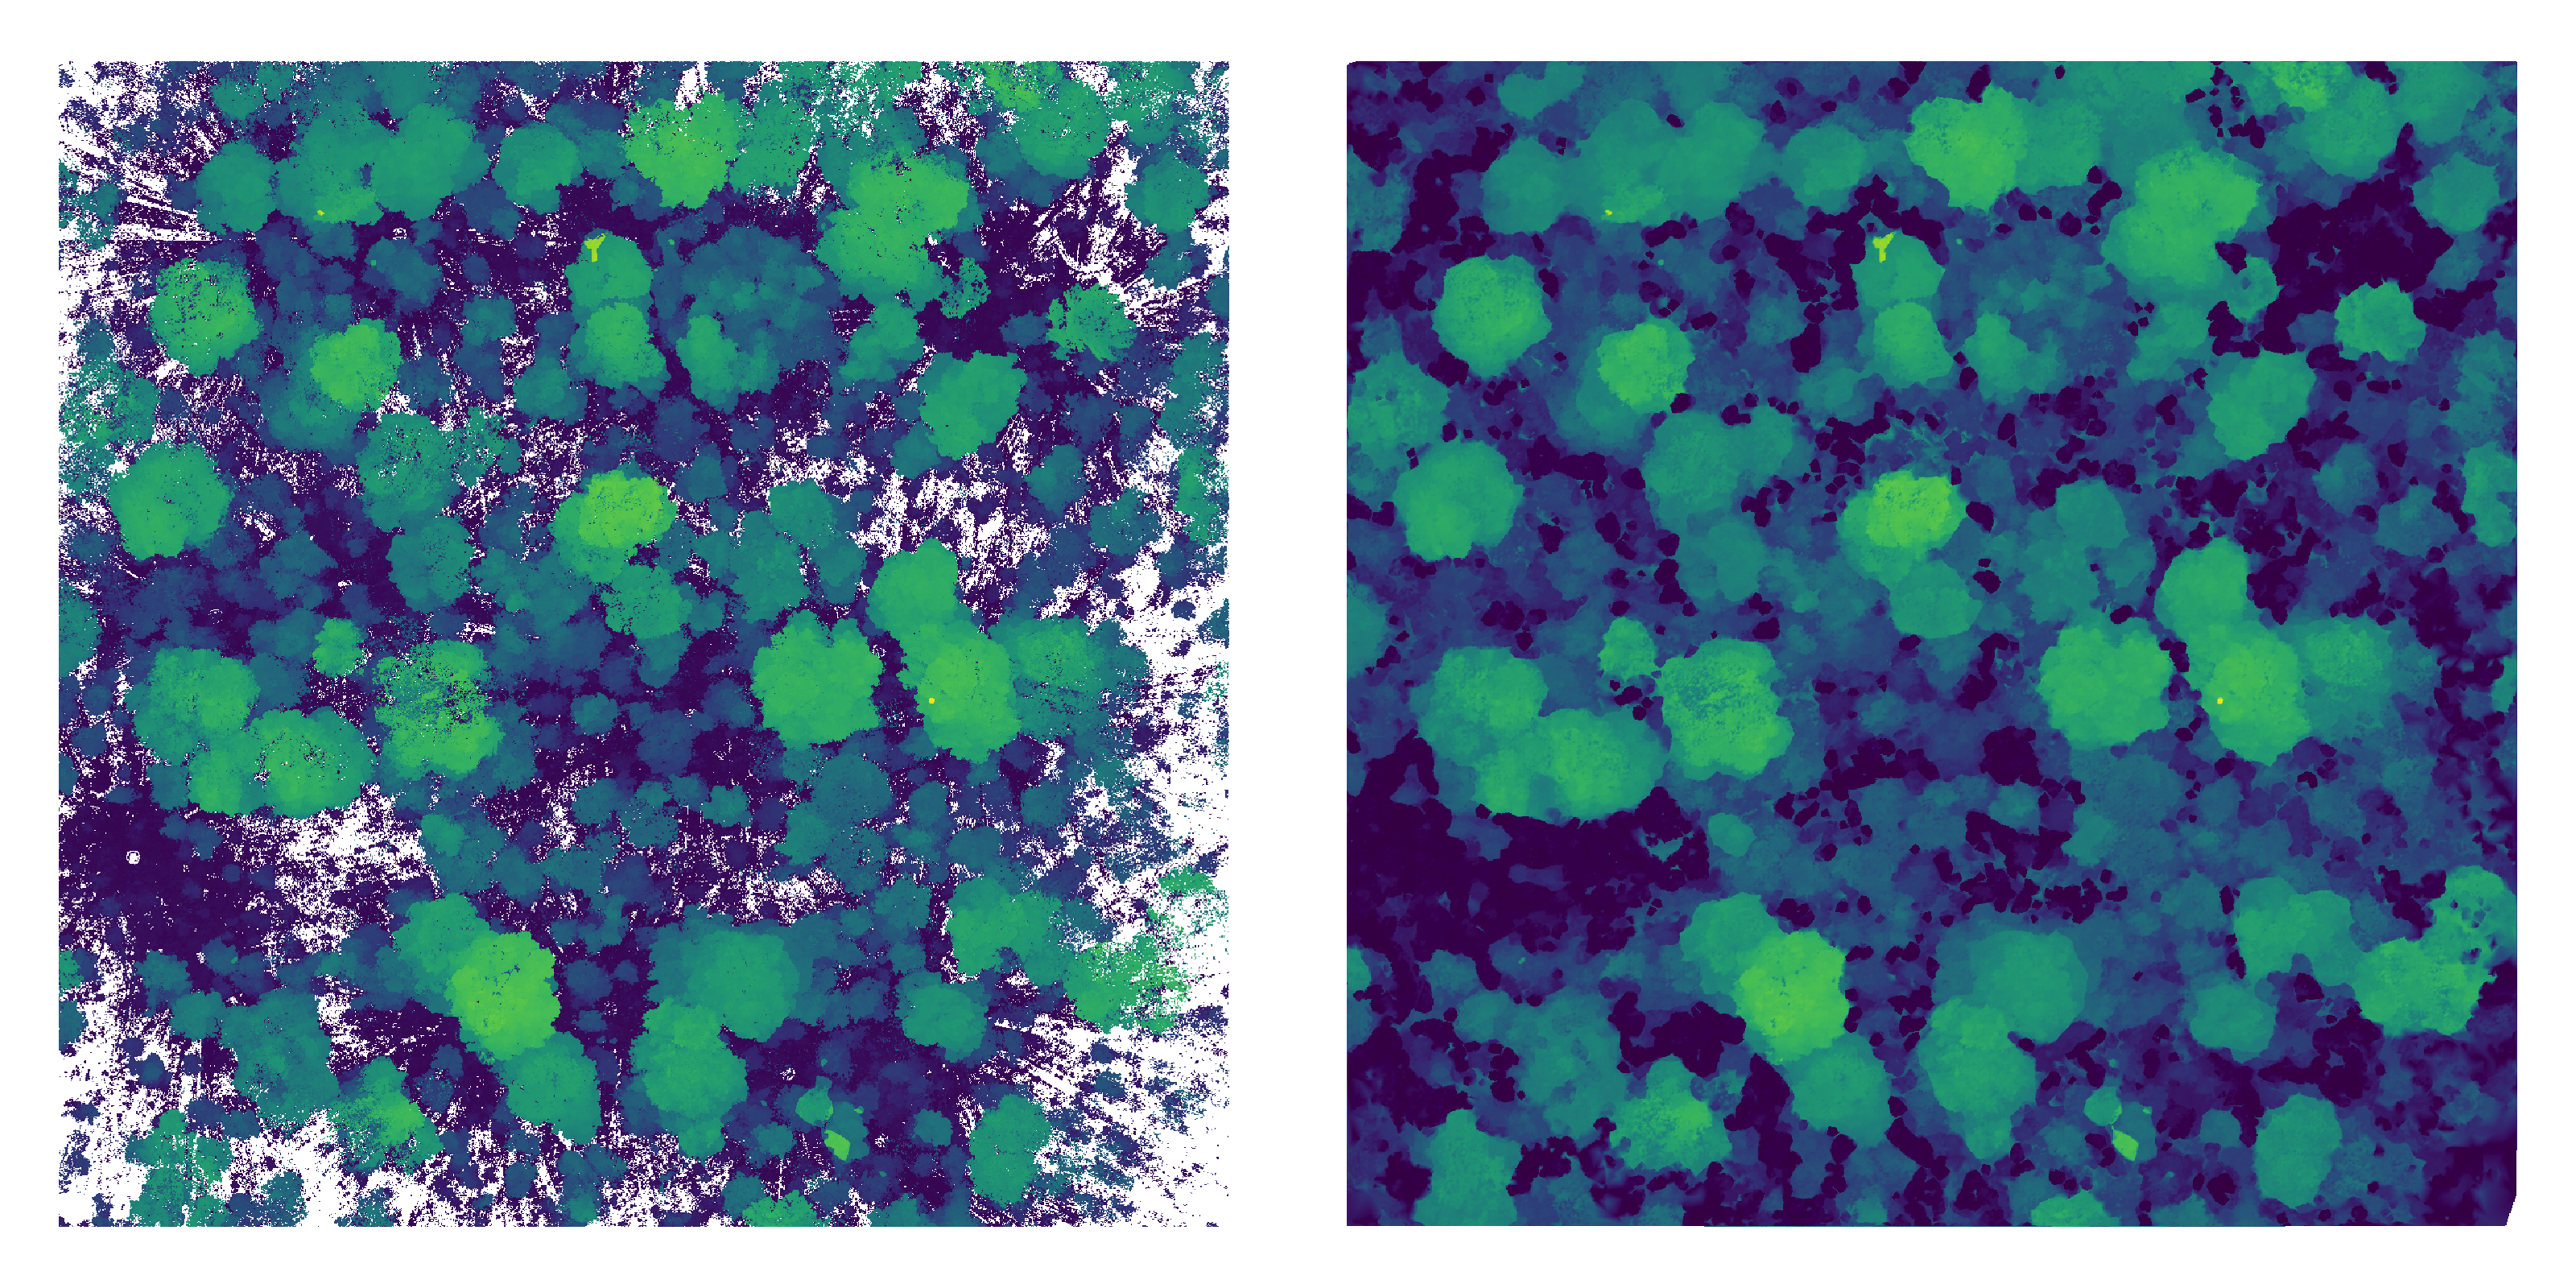
\includegraphics[width=\textwidth]{P1_both}
	\caption{Top-down view of a 1 ha plot in Bicuar National Park. a) shows the point cloud after voxelisation, noise reduction, and taking the 99th percentile of stem height in each 5 cm vertical bin. b) shows the same point cloud after pit filling to generate a smooth canopy height profile. Points are coloured according to point height from the ground.}
	\label{P1_both}
\end{figure}

From the canopy height profile we extracted a number of statistics for use in statistical modelling. We calculated the mean and coefficient of variation of canopy height across the plot (canopy rugosity), following \citep{Parker2004}. We calculated the Topographic Ruggedness Index (TRI) as the mean of absolute differences between the heights of each column and the height of its eight surrounding cells \citep{Wilson2007}. From this we estimated the plot level mean TRI and coefficient of variation. 

We also calculated a second measure of canopy rugosity ($R_{c}$) that considers the entire canopy profile, rather than just the canopy top, following \citet{Hardiman2011}

\begin{equation}
	R_{c} = \sigma{}(\sigma{}G_{z})_{x}
\end{equation}

Where $G_{z}$ is the vertical height axis $z$, $x$ is the horizontal axis, and $\sigma{}$ is the standard deviation.

\section{Statistical analysis}

All linear mixed effects models werre conducted using the \texttt{\{lmer\}} package in R version 4.0.2 \citep{R2021}.

\subsection{Foliage density profiles}

We conducted a number of linear mixed effects models to assess the effects of tree diversity and stand structure on various aspects of canopy structure measured at the 10 m subplot scale. Linear mixed effects models were used to account for the non-independence of samples caused by the nested sampling structure of subplots within plots, and plots within sites. For each subplot canopy structure measure, we created a linear mixed effects model with fixed effects of subplot species richness, and tree spatial structure using the adapted Hegyi index ($H_{i}$) and the coefficient of variation of stem diameter. We compared the standardized effect sizes of each fixed effect to understand the relative effect of species richness and spatial structure on canopy structure. We compared models with all combinations of fixed effects to understand which combination of fixed effects best explained variation in each subplot canopy structure measure. We also compared models to a null model including only random effects of plot and site to evaluate whether this `best' model explained real variation in canopy structure.

\subsection{Grass biomass}

To estimate the correlation between grass volume estimated by TLS and grass biomass estimated from the allometry of DPM height and grass biomass samples, we conducted a linear mixed effects model of grass biomass vs. grass volume, with nested random slope terms for each 1 ha plot nested within site. 

We conducted a linear mixed effects model to assess the effects of canopy structure on grass volume, with random slope terms for each 1 ha plot nested within site. We began with a maximal model which included fixed effects of subplot tree species richness, stem density, TLS canopy cover, layer diversity, height of maximum foliage density, standard deviation of the foliage density profile, and our simple measure of foliage density uniformity. We re-fitted the model with all possible combinations of fixed and random effects and compared AIC, BIC, and log-likelihood to determine which combination of explanatory variables best accounted for variation in grass volume. Once this `best model' had been identified we extracted standardized effect sizes for each fixed effect to compare their relative contribution to the model. We also compared random effects for each fixed effect to understand how the relationship differed between the two sites.

\subsection{Canopy rugosity}

To understand the effect of species composition and stand structure on whole-plot canopy rugosity, we conducted a linear mixed effects model with fixed effects of tree species shannon diversity index, stem density, spatial mingling index and winkelmass, with random intercept terms for each site. We extracted slopes for each fixed effect to compare their effect sizes and compared our model with a null model which consisted only of the random effect of site and the fixed effect of stem density.

\printbibliography

\end{document}

